\label{benchmarkdata}
\section{Benchmark Data}
\begin{table}[h]
	\centering
	\begin{tabular}{ll|l|l|l|l|l}
		Server      & Version & Method & N  & Mean    & Error  & StdDev \\ \hline
		Nano Server & 1709    & SHA256 & 10 & 769.900 & 11.909 & 9.945  \\
		Nano Server & 1709    & MD5    & 10 & 516.500 & 8.543  & 7.991  \\
		Nano Server & 1809    & SHA256 & 10 & 781.800 & 13.820 & 12.930 \\
		Nano Server & 1809    & MD5    & 10 & 513.700 & 10.950 & 11.240 \\
		Server Core & 1709    & SHA256 & 10 & 813.900 & 16.370 & 23.478 \\
		Server Core & 1709    & MD5    & 10 & 502.300 & 9.554  & 8.937  \\
		Server Core & 1809    & SHA256 & 10 & 777.900 & 13.352 & 18.275 \\
		Server Core & 1809    & MD5    & 10 & 516.500 & 9.911  & 9.734  \\
		Windows     & 1809    & SHA256 & 10 & 854.200 & 16.730 & 20.543 \\
		Windows     & 1809    & MD5    & 10 & 571.100 & 11.110 & 9.844  \\
		Nano Server & 1709    & SHA256 & 20 & 796.300 & 12.101 & 11.320 \\
		Nano Server & 1709    & MD5    & 20 & 517.400 & 10.550 & 13.465 \\
		Nano Server & 1809    & SHA256 & 20 & 797.800 & 16.060 & 18.490 \\
		Nano Server & 1809    & MD5    & 20 & 531.000 & 10.450 & 14.650 \\
		Server Core & 1709    & SHA256 & 20 & 772.400 & 14.251 & 11.901 \\
		Server Core & 1709    & MD5    & 20 & 503.400 & 9.842  & 12.798 \\
		Server Core & 1809    & SHA256 & 20 & 777.200 & 13.499 & 11.272 \\
		Server Core & 1809    & MD5    & 20 & 508.400 & 10.182 & 10.895 \\
		Windows     & 1809    & SHA256 & 20 & 831.700 & 13.110 & 11.620 \\
		Windows     & 1809    & MD5    & 20 & 568.700 & 15.020 & 17.882
	\end{tabular}
	\label{BenchmarkData}
	\caption{Benchmarking Results}
\end{table}
\section{Graphs}
\begin{figure}[h]
	\captionsetup{width=0.8\linewidth}
	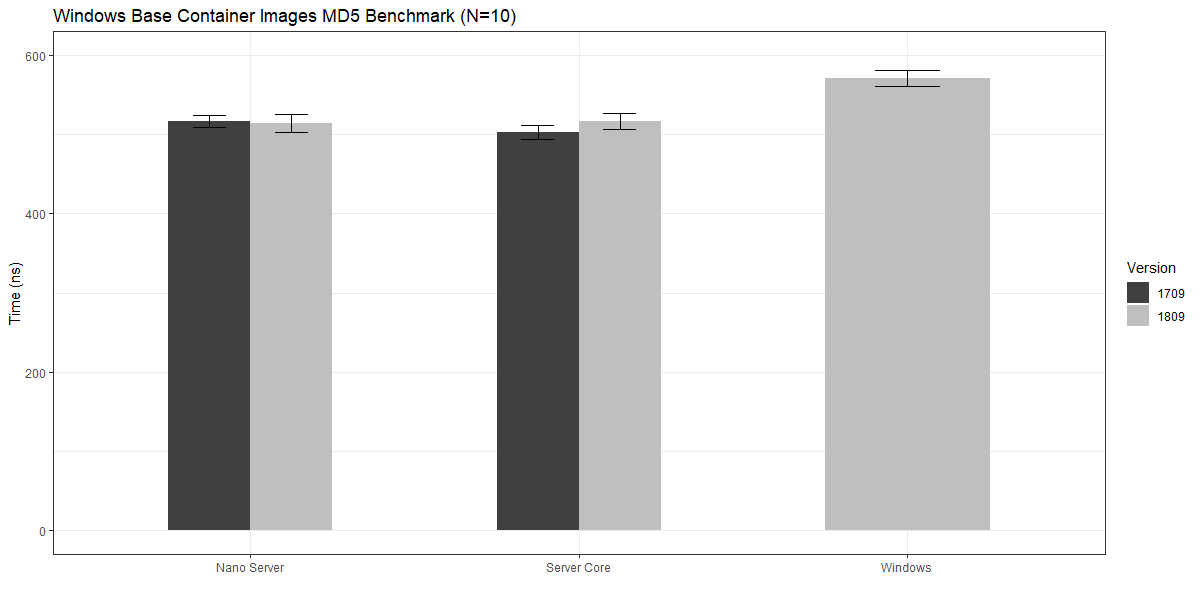
\includegraphics[width=0.9\linewidth]{img/MD5_10.png}
	\centering
	\caption{Windows Base Container Image MD5 Benchmark (N=10)}
	\label{fig:MD5_10}
\end{figure}
\begin{figure}[h]
	\captionsetup{width=0.8\linewidth}
	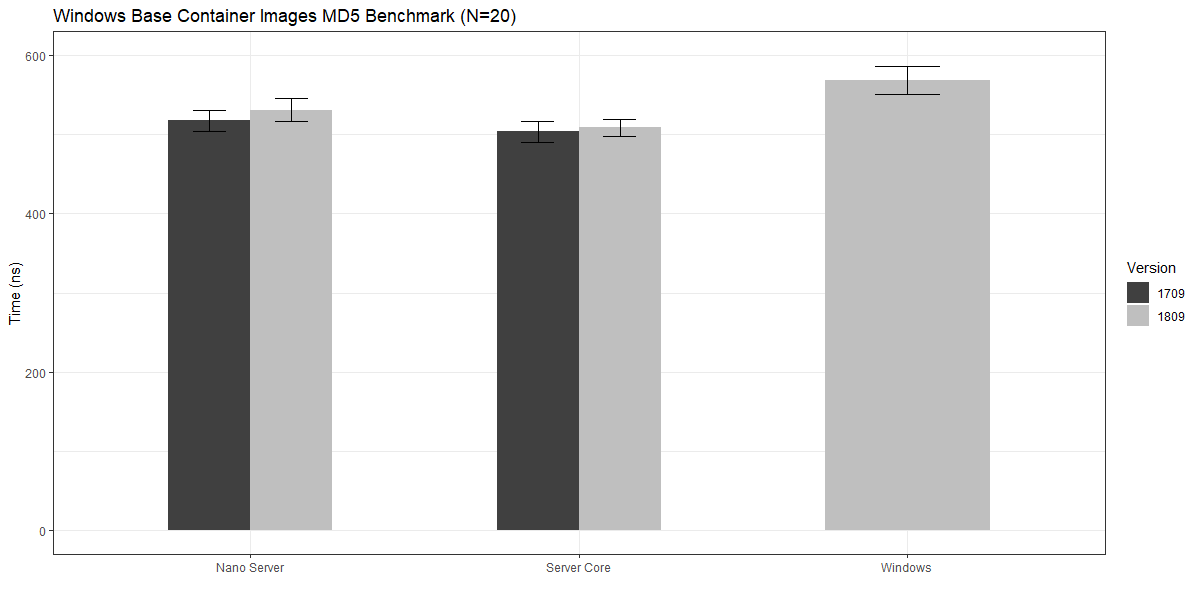
\includegraphics[width=0.9\linewidth]{img/MD5_20.png}
	\centering
	\caption{Windows Base Container Image MD5 Benchmark (N=20)}
	\label{fig:MD5_20}
\end{figure}
\begin{figure}[h]
	\captionsetup{width=0.8\linewidth}
	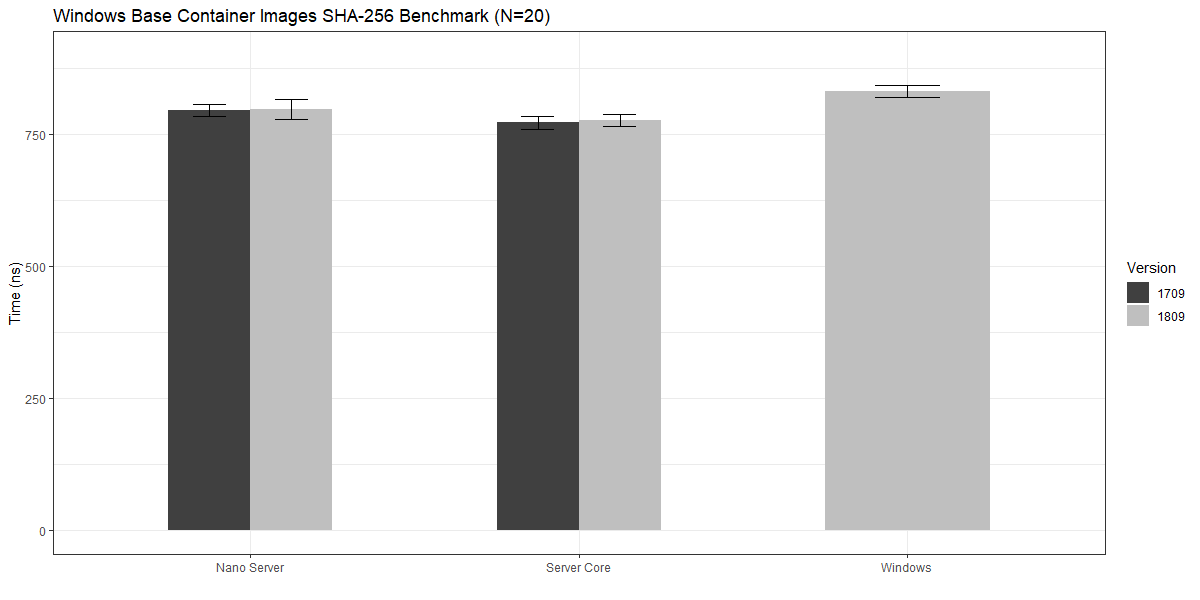
\includegraphics[width=0.9\linewidth]{img/SHA_20.png}
	\centering
	\caption{Windows Base Container Image SHA-256 Benchmark (N=10)}
	\label{fig:SHA_10}
\end{figure}
\begin{figure}[h]
	\captionsetup{width=0.8\linewidth}
	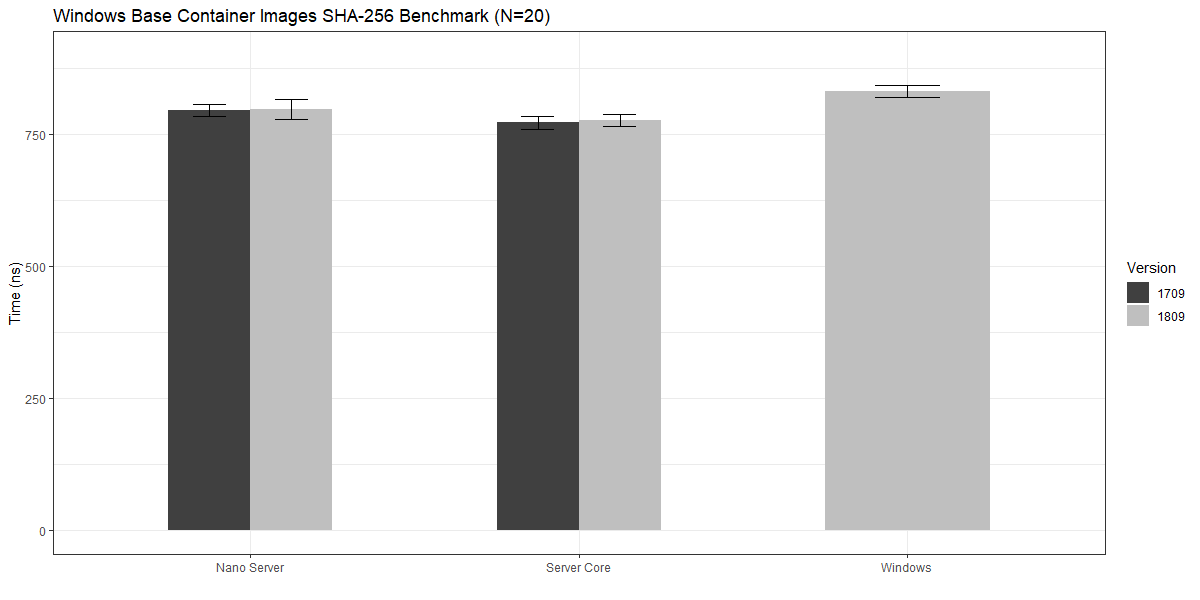
\includegraphics[width=0.9\linewidth]{img/SHA_20.png}
	\centering
	\caption{Windows Base Container Image SHA-256 Benchmark (N=20)}
	\label{fig:SHA_20}
\end{figure}